\documentclass[a4paper]{article}

\usepackage{amsmath,amssymb}
\usepackage[dvipdfmx]{graphicx}

\textwidth \paperwidth
\addtolength{\textwidth}{-1.8in}
\oddsidemargin -0.1in
\marginparsep 0pt
\marginparwidth 0pt
\hoffset 0pt

\textheight \paperheight
\addtolength{\textheight}{-2in}
\topmargin 0pt
\headheight 0pt
\headsep 0pt
\footskip 0.3in
\voffset 0pt

\begin{document}

\section*{Mathematical descriptions of Fourier Symmetrization}
The Fourier symmetrization consists of two steps.
One is correcting distortion of an original FFT image, and the other is folding and rotating a corrected image based on a crystal symmetry.
This note gives mathematical descriptions about each step.

\subsection*{Correcting distortion}
An FFT image is usually distorted due to various reasons such as piezo creep, thermal drift, and difference of piezo constants in $x$ and $y$ directions.
This section describes mathematical basis of correcting such distortion.
Here we think about uniform distortion constant in time: expansion, shrinkage, and shear in $x$ and $y$ directions (Fig.~\ref{fig:distortion}).
Such distortion results in deviation of FFT peak locations from ideal ones.
Our goal is to find how to correct the deviation.
\begin{figure}[h]
	\begin{center}
		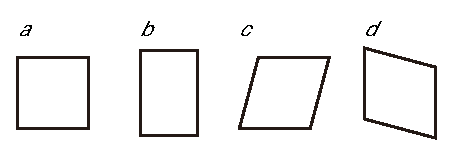
\includegraphics[keepaspectratio]{distortion.eps}
	\end{center}
	\caption{Distortion. (a) ideal, (b) expansion and shrinkage, (c) $x$-shear, (d) $y$-shear.}
	\label{fig:distortion}
\end{figure}

Let coordinates of atomic peaks observed in an FFT image $\boldsymbol{q}_1 = (q_{1x}, q_{1y})$ and $\boldsymbol{q}_2 = (q_{2x}, q_{2y})$.
Due to the distortion, these peaks are shifted from the ideal locations, ${\boldsymbol{q}_1}^\prime$ and ${\boldsymbol{q}_2}^\prime$.
This shift is expressed by a $2\times 2$ matrix $M$, ${\boldsymbol{q}_i}^\prime = M\boldsymbol{q}_i$.
Our goal is nothing but getting the matrix $M$.

When shear direction is $x$, $M$ is given as a product of matrices of shear and expansion (or shrinkage),
\begin{equation}
M=\left(
\begin{array}{cc}
m_1 & m_2 \\
0 & m_3
\end{array}
\right)=\left(
\begin{array}{cc}
1 & m_2/m_3 \\
0 & 1
\end{array}
\right)\left(
\begin{array}{cc}
m_1 & 0 \\
0 & m_3
\end{array}
\right).
\label{eq:mx}
\end{equation}
To get these three parameters of $M$, we solve the following three equations: $|{\boldsymbol{q}_i}^\prime|=1/a_i$ and ${\boldsymbol{q}_1}^\prime\cdot{\boldsymbol{q}_2}^\prime=|{\boldsymbol{q}_1}^\prime||{\boldsymbol{q}_2}^\prime|\cos\theta$, where $a_i$ is the distance\footnote{This is the $d$ value in terms of X-ray diffraction. It depends on the symmetry of lattice whether this is the same as the lattice constant $a_0$. For example, $a_i=a_0$ for 4mm and $a_i = \sqrt{3}a_0/2$ for 3m.} between atomic rows corresponding to $\boldsymbol{q}_i$ and $\theta$ is the angle between ${\boldsymbol{q}_1}^\prime$ and ${\boldsymbol{q}_2}^\prime$ determined by a crystal symmetry.
Given ${\boldsymbol{q}_i}^\prime = M\boldsymbol{q}_i$, these three equations are
\begin{equation}
(q_{1x}m_1+q_{1y}m_2)^2+(q_{1y}m_3)^2 = 1/{a_1}^2,
\end{equation}
\begin{equation}
(q_{2x}m_1+q_{2y}m_2)^2+(q_{2y}m_3)^2 = 1/{a_2}^2,
\end{equation}
\begin{equation}
(q_{1x}m_1+q_{1y}m_2)(q_{2x}m_1+q_{2y}m_2)+q_{1y}q_{2y}{m_3}^2 = \cos\theta/(a_1a_2).
\end{equation}
These equations can be rewritten as
\begin{equation}
\left(
\begin{array}{ccc}
{q_{1x}}^2 & 2q_{1x}q_{1y} & {q_{1y}}^2 \\
{q_{2x}}^2 & 2q_{2x}q_{2y} & {q_{2y}}^2 \\
q_{1x}q_{2x} & q_{1x}q_{2y}+q_{2x}q_{1y} & q_{1y}q_{2y} 
\end{array}
\right)\left(
\begin{array}{c}
A\\B\\C
\end{array}
\right)=\left(\!
\begin{array}{c}
1/{a_1}^2\\
1/{a_2}^2\\
\cos\theta/(a_1a_2)
\end{array}
\right),
\label{eq:main}
\end{equation}
where $A = {m_1}^2, B = m_1m_2,$ and $C = {m_2}^2+{m_3}^2$.

When shear direction is $y$, $M$ is given as
\begin{equation}
M=\left(
\begin{array}{cc}
m_1 & 0 \\
m_2 & m_3
\end{array}
\right)=\left(
\begin{array}{cc}
1 & 0 \\
m_2/m_1 & 1
\end{array}
\right)\left(
\begin{array}{cc}
m_1 & 0 \\
0 & m_3
\end{array}
\right).
\label{eq:my}
\end{equation}
We can get equations for $y$-shear case in the same manner to get Eq.~(\ref{eq:main}).
The resultant equations have the same form as Eq.~(\ref{eq:main}), but $A = {m_1}^2+{m_2}^2, B = m_2m_3,$ and $C = {m_3}^2$.

Now we find that equations to be solved are Eq.~(\ref{eq:main}) with respect to $A$, $B$, and $C$.
By solving the equations, we finally get the matrix as
\begin{equation}
m_1 = \sqrt{A},\quad m_2 = \frac{B}{\sqrt{A}},\quad m_3 = \sqrt{C-\frac{B^2}{A}}\qquad{\rm (for\ }x{\rm -shear)},
\end{equation}
\begin{equation}
m_1 = \sqrt{A-\frac{B^2}{C}},\quad m_2 = \frac{B}{\sqrt{C}},\quad m_3 = \sqrt{C}\qquad{\rm (for\ }y{\rm -shear)},
\end{equation}
where
\begin{align}
A &= \frac{{q_{2y}}^2/{a_1}^2+{q_{1y}}^2/{a_2}^2-2q_{1y}q_{2y}\cos\theta/(a_1a_2)}{(q_{1x}q_{2y}-q_{1y}q_{2y})^2},\\
B &= -\frac{q_{2x}q_{2y}/{a_1}^2+q_{1x}q_{1y}/{a_2}^2-(q_{1x}q_{2y}+q_{1y}q_{2x})\cos\theta/(a_1a_2)}{(q_{1x}q_{2y}-q_{1y}q_{2y})^2},\\
C &= \frac{{q_{2x}}^2/{a_1}^2+{q_{1x}}^2/{a_2}^2-2q_{1x}q_{2x}\cos\theta/(a_1a_2)}{(q_{1x}q_{2y}-q_{1y}q_{2y})^2}.
\end{align}

In actual process with Igor Pro, the wave scaling is changed to correct expansion or shrinkage in $x$ and $y$ directions ($m_1$ and $m_3$).
You may want to change aspect ratio of a window to plot a symmetrized FFT image.
Parameters used to correct distortion ($m_1$, $m_2$, and $m_3$) are saved as wave note of a resultant symmetrized wave.

\subsection*{Folding and rotating an FFT image}

Folding and rotating an FFT image are done based on mirror and rotational symmetries of a crystalline lattice, respectively.
Important properties of an FFT image for this purpose are that amplitude of an FFT image has
\begin{enumerate}
	\item mirror symmetry same as that of an original real-space image,
	\item rotational symmetry same as that of an original real-space image,
	\item $C_2$ symmetry.
\end{enumerate}
We make sure these properties in the following sections.
Let $f(x,y)$ and $F(q_x,q_y)$ are a real-space image and its Fourier transform, respectively,
\begin{equation}
	F(q_x,q_y) = \int f(x,y)e^{-i(q_xx+q_yy)}dxdy.
\end{equation}

\subsubsection*{mirror symmetry}
When $f(x,y)$ has mirror symmetry with respect to $x$-axis, $f(x,y)=f(-x,y)$,
\begin{align}
	F(q_x,q_y) &= \int f(-x,y)e^{-i(q_xx+q_yy)}dxdy\\
		&= -\int f(x,y)e^{-i(-q_xx+q_yy)}dxdy\\
		&= -F(-q_x,q_y).
\end{align}
Therefore, $|F(q_x,q_y)|=|F(-q_x,q_y)|$.

\subsubsection*{rotational symmetry}
When $f(x,y)$ has rotational symmetry, $f(x,y)=f(x\cos\theta-y\sin\theta,x\sin\theta+y\cos\theta)$,
\begin{align}
	F(q_x,q_y) &= \int f(x\cos\theta-y\sin\theta,x\sin\theta+y\cos\theta)e^{-i(q_xx+q_yy)}dxdy\\
		&= \int f(x,y)e^{-i(q_x(x\cos\theta+y\sin\theta)+q_y(-x\sin\theta+y\cos\theta))}dxdy\\
		&= F(q_x\cos\theta-q_y\sin\theta,q_x\sin\theta+q_y\cos\theta).
\end{align}

\subsubsection*{$C_2$ symmetry}
Since $f(x,y)$ is a real function,
\begin{align}
	F^*(q_x,q_y) &= \int f^*(x,y)e^{i(q_xx+q_yy)}dxdy\\
		&= \int f(x,y)e^{-i(-q_xx-q_yy)}dxdy\\
		&= F(-q_x,-q_y).
\end{align}
Therefore, $|F(q_x,q_y)|=|F(-q_x,-q_y)|$.

\subsubsection*{Symmetrization}
Fig.~\ref{fig:symmetry} shows equivalent points in FFT space, which are averaged by symmetrization.
$p$3m1 and $p$31m have different sets of equivalent points.
Due to $C_2$ symmetry described above, however, eventually they have the same set of equivalent points.
Consequently, atomic peaks can be available to indicate high-symmetry direction for all symmetries.
Half of the equivalent points are used for actual calculation to reduce amount of calculation.
Effective multiplicity is 2, 6, and 4 for 2mm, 3m, and 4mm, respectively.

\begin{figure}[h]
	\begin{center}
		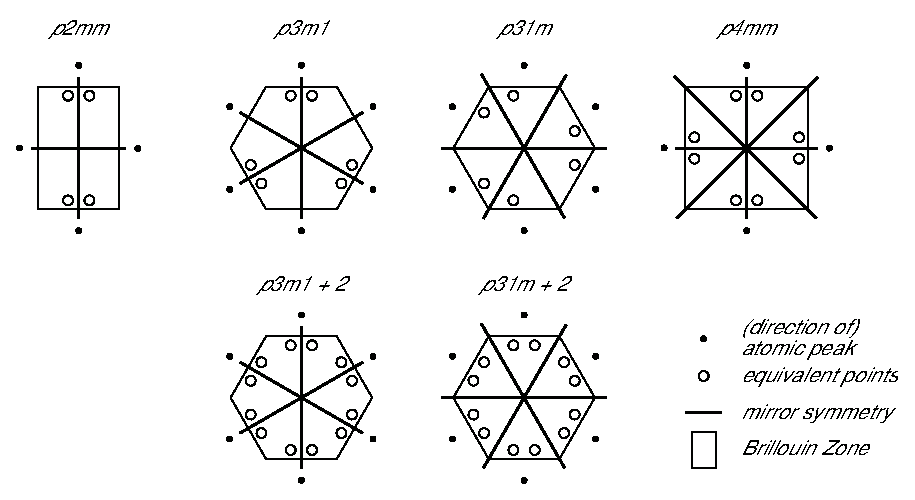
\includegraphics[keepaspectratio]{symmetry.eps}
	\end{center}
	\caption{Equivalent points in FFT space for each symmetry.}
	\label{fig:symmetry}
\end{figure}

\end{document}